\documentclass[14pt]{extarticle}
\usepackage{afterpage}
\usepackage{amsmath}
\usepackage{amssymb}
\usepackage{bbm}
\usepackage[legalpaper,left=3cm,right=1.5cm,top=2cm,bottom=2cm]{geometry}
\usepackage{graphicx}
\usepackage[utf8]{inputenc}
\usepackage[T1, T2A]{fontenc}
\usepackage[english,russian]{babel}
\usepackage{pdflscape}

\bibliographystyle{unsrt}

\DeclareMathOperator{\diag}{diag}
\DeclareMathOperator{\Arg}{Arg}
\DeclareMathOperator{\Tr}{Tr}

\newcommand{\bra}{\langle}
\newcommand{\ket}{\rangle} 

\graphicspath{ {images/} }

\begin{document}
    \begin{titlepage}
	\centering
	{\scshape\LARGE Московский физико--технический институт\par}
	{\scshape Кафедра проблем физики и астрофизики \par}
	\vspace{1cm}
	{\scshape\Large Отчёт о научной работе за 2 семестр 2016--2017 учебного года\par}
	\vspace{1.5cm}
	{\huge\bfseries Стабильность краевых состояний в топологических изоляторах
        \par}

	\vspace{2cm}
	{\Large\itshape Аникин Евгений\par}
	\vfill
	научный руководитель\par
	чл.-к.~РАН~д.~ф--м.~н.~П.И. \textsc{Арсеев}

	\vfill

% Bottom of the page
	{\large \today\par}
\end{titlepage}

    \tableofcontents
    	\newpage
%	\begin{abstract}
%        Из модели сильной связи для полупроводника с сильным спин--орбитальным
%        расщеплением выведен эффективный гамильтониан квантовой ямы.
%        Показано, что этот гамильтониан описывает топологический изолятор.
%        Для эфективного гамильтониана найден спектр одиночной примеси.
%	\end{abstract}
	\section{Введение}
    Двумерные топологические изоляторы --- это двумерные кристаллы 
    с особого рода зонной структурой:
    в них невозможно однозначно задать фазу функций 
    Блоха во всей зоне Бриллюэна. Причина этого в том, что (в простейшем случае) 
    отличен от нуля
    топологический инвариант \cite{Kohmoto1985}
    \begin{equation}
        \label{TKNN}
        N = \frac{1}{2\pi i} 
            \int d^2 k\, \left[\partial_i \langle u | \partial_j u \rangle -
            \partial_j \langle u | \partial_i u \rangle \right]
    \end{equation}
    В реалистичном случае этот инвариант отличен от нуля для каждой из компонент спина,
    но имеет для них противоположные знаки.
    Этот инвариант определяет спин--холловскую проводимость, 
    измеренную в квантах 
    магнитного потока:
    \begin{equation}
        \sigma_{xy} = \frac{e^2}{2\pi \hbar} N
    \end{equation}
    
    Наконец, точно так же, как в эффекте Холла, 
    на границе топологических изоляторов всегда возникают краевые состояния,
    пересекающие запрещённую зону, см. \cite{Hasan2010}.

    Эти краевые состояния обладают свойством киральности: электроны со спином 
    вверх движутся в одну сторону, а со спином вниз --- в другую. Кроме того, состояния 
    с разным направлением движения составляют крамерсовский дублет. Поэтому
    эти состояния не могут рассеиваться друг в друга 
    под действием какого--либо возмущения, то есть граница топологического 
    изолятора представляет из себя идеальный одномерный проводник.

    В многочисленных экспериментах (например, \cite{Konig2007}, \cite{Gusev2011})
    показано, что квантовая яма HgTe является топологическим изолятором при 
    некоторых параметрах. Наличие краевых состояний подтверждается измерениями
    нелокального сопротивления. Однако, хотя краевые состояния и
    определяют транспорт в квантовой яме, этот транспорт оказывается не баллистическим 
    \cite{Gusev2011}.
    Поэтому представляют интерес механизмы, которые могут приводить
    к рассеянию краевых мод друг в друга, либо иные механизмы, приводящие к неидеальности
    краевого транспорта.

    Целью настоящей работы является исследование влияние глубоких примесей на краевой 
    транспорт. Имеются в виду такие примеси, для которых энергия связанного состояния
    лежит внутри щели. Это, казалось бы, открывает возможность переходов краевых
    состояний в примесные и наоборот, и может приводить к изменению проводимости.
    

%#    Целью настоящей работы является изучение нескольких механизмов, которые
%#    потенциально могут приводить к рассеянию краевых состояний. Мы рассмотрели 
%#    точечную примесь в топологическом изоляторе, нашли для неё связанные состояния 
%#    и обсудили возможность образования примесных уровней в запрещённой зоне. 
%#    (Похожие вещи обсуждались в \cite{Lu2011}. Также 
%#    методом прямой диагонализации показана устойчивость краевых состояний к сильным
%#    потенциальным примесям и, наоборот, локализация магнитным беспорядком. Наконец, 
%#    обсуждается возможность спонтанного нарушения симметрии около края, вследствие чего
%#    краевые состояния перестают быть защищёнными. Все вычисления проделаны в эффективной
%#    модели сильной связи, описывающей два уровня размерного квантования квантовой ямы
%#    HgTe. 
    
%    Топологические изоляторы реализованы экспериментально в квантовых ямах $HgTe$. 
%    Теллурид ртути --- узкозонный полпроводник, 
%    Только системы со спин--орбитальным 
%    взаимодействием могут быть топологическими изоляторами. Впервые 
%    Дело в том, что холловская проводимость неинвариантна по отношению к обращению
%    времени, поэтому в системе с $\mathrm{T}$--симметрией, каковой является кристалл 
%    при отсутствии магнитного поля, и при от отсутствии спин--орбитального взаимодействия
%    $N$ обязательно равно нулю. Иная ситуация возникает, когда есть
%    спин--орбитальное взаимодействие. В этом случае $N$ может быть отлично от нуля
%    для каждой из компонент спина. 

    


    

    \section{Топологический изолятор на основе квантовой ямы HgTe}
    

    \section{Квантовая яма CdTe--HgTe--CdTe\\ в модели сильной связи}
В этом разделе будет построена модель сильной связи, эквивалентная $k\cdot p$ гамильтониану
\eqref{kane_ham}. Численно диагонализуя её, можно независимо получить уровни размерного 
квантования.
\subsection{Модель однородного полупроводника}
Модель представляет из себя 
кубическую решётку из атомов, на каждом из которых ``сидят'' состояния
с $p_x$, $p_y$, $p_z$ и $s$--орбиталями и двумя 
возможными проекцими спина.

Для написания
спин--орбитального гамильтониана $p$--зоны необходимо перейти к состояниям с определённым
полным моментом. Эти состояния выражаются через $p_x$, $p_y$, $p_z$ орбитали через
коэффициенты Клебша--Гордана.

Спин--орбитальное взаимодействие приводит к расщеплению состояний с моментами $\frac32$ и
$\frac12$.
Состояниями с полным моментом $\frac{1}{2}$ 
можно пренебречь, если спин--орбитальное взаимодейтвие велико. Таким образом, в каждом
узле решётки остаётся пара $s$--орбиталей, формирующая валентную зону, и четыре состояния
с полным моментом $\frac{3}{2}$. Матричные элементы перекрытия между состояниями на соседних
узлах выражаются через перекрытия $s$ и $p$ орбиталей с использованием их выражений через
коэффициенты Клебша--Гордана.

Определим матричные элементы $t_\parallel$ и $t_\perp$ для перекрытия соседних $p$--орбиталей,
расположенных соответственно <<вдоль>> и <<поперёк>>, $\frac{-iP}{2}$ для перекрытия
$s$ и $p$--орбитали и $-\frac{1}{2m_s}$ --- для $s$--орбиталей. Через них полный гамильтониан
сильной связи записывается в импульсном представлении в виде огромной матрицы $6\times6$. 

\begin{equation}
    \label{hfull}
    H_{\mathrm{full}} = \begin{pmatrix}
                            H_c & T \\
                            T^\dagger & H_v
                        \end{pmatrix},
\end{equation}
Матрицы $H_c$, $T$, $H_v$ определены формулами \eqref{H_conduction}--\eqref{H_valence}, см.
стр.~\pageref{H_conduction}.
Этот гамильтониан можноразложить по малым $p$,
в результате чего получится гамильтониан Латтинжера:
\begin{equation}
    H_v = \frac{\hbar^2}{2ma^2}\left\{-\left(\gamma_1 + \frac{5}{2}\gamma_2\right) k^2 + 
        2\gamma_2(k_x^2J_x^2 + k_y^2J_y^2 + k_z^2J_z^2) + 
        4\gamma_3(k_x k_y J_x J_y + k_x k_z J_x J_z + k_y k_z J_y J_z) \right\}
\end{equation}
Здесь $J_i$ --- операторы момента для спина $\frac{3}{2}$, $a$ --- постоянная решётки,
$m$ --- масса электрона,
\begin{equation}
    \begin{gathered}
        \frac{\hbar^2}{2ma^2}\gamma_1 = \frac13 t_\parallel\\
        \frac{\hbar^2}{2ma^2}\gamma_2 = \frac16(t_\parallel - t_\perp)\\
        \gamma_3 = 0\\
    \end{gathered}
\end{equation}
Разложение $H_c$ и $T$ тривиально.
Всё это вместе воспроизводит модель Кейна, которую обычно получают в $k \cdot p$ приближении.

Коэффициенты перескока в сильной связи можно зафиксировать требованием, чтобы при малых $p$ 
воспроизводился $k\cdot p$ гамильтониан с значениями параметров, известных из эксперимента
\cite{Novik2005}. 

%\section{Коэффициенты Клебша--Гордана}
%\label{app:tb}
%Состояния с определённым полным моментом выражаются через $p_x$, $p_y$, $p_z$ орбитали через
%коэффициенты Клебша--Гордана:
%\begin{equation}
%	\label{transform1}
%	\begin{gathered}
%        \Psi_{\frac{3}{2},\frac{3}{2}} = \frac{X + iY}{\sqrt{2}}\alpha\\
%        \Psi_{\frac{3}{2}, \frac{1}{2}} = \sqrt{\frac{1}{3}}\frac{X + iY}{\sqrt{2}}\beta -
%                                         \sqrt{\frac{2}{3}} Z\alpha\\
%        \Psi_{\frac{3}{2}, -\frac{1}{2}} = -\sqrt{\frac{1}{3}}\frac{X - iY}{\sqrt{2}}\alpha -
%                                         \sqrt{\frac{2}{3}} Z\beta\\
%        \Psi_{\frac{3}{2},-\frac{3}{2}} = -\frac{X - iY}{\sqrt{2}}\beta
%	\end{gathered}
%\end{equation}
%\begin{equation}
%	\label{transform2}
%	\begin{gathered}
%        \Psi_{\frac{1}{2}, \frac{1}{2}} = \sqrt{\frac{2}{3}}\frac{X + iY}{\sqrt{2}}\beta +
%                                         \sqrt{\frac{1}{3}} Z\alpha\\
%        \Psi_{\frac{1}{2}, -\frac{1}{2}} = -\sqrt{\frac{2}{3}}\frac{X - iY}{\sqrt{2}}\alpha-
%                                         \sqrt{\frac{1}{3}} Z\beta\\
%	\end{gathered}
%\end{equation}
%
%Здесь $X,Y,Z$ --- атомные орбитали, $\alpha,\beta$ --- состояния со спином вверх и вниз.

\afterpage{%
    \clearpage% Flush earlier floats (otherwise order might not be correct)
%    \thispagestyle{empty}% empty page style (?)
    \begin{landscape}% Landscape page
        \centering % Center table
        \vspace*{\fill}
        \begin{equation}
            \label{H_conduction}
            H_c = (E_s + \frac{1}{m_s}(3 - \cos{p_x} - \cos{p_y} - \cos{p_z}))I_{2\times2}
        \end{equation}
        \begin{equation}
            \label{T_matrix}
            T = P\begin{pmatrix}
                    -\frac{1}{\sqrt{2}}(\sin{p_x} + i\sin{p_y}) & \sqrt{\frac{2}{3}}\sin{p_z} &
                     \frac{1}{\sqrt{6}}(\sin{p_x} - i\sin{p_y}) & 0 \\  
                    0 & -\frac{1}{\sqrt{6}}(\sin{p_x} + i\sin{p_y}) & 
                    \sqrt{\frac{2}{3}}\sin{p_z} & \frac{1}{\sqrt{2}}(\sin{p_x} - i\sin{p_y}),
                 \end{pmatrix},
        \end{equation}
        \begin{equation}
            \label{H_valence}
            H_v = 
            \begin{pmatrix}
                (t_\parallel + t_\perp)(\cos{p_x} + \cos{p_y}) + 2t_\perp \cos{p_z} & 0 &
                -\frac{1}{\sqrt{3}}(t_\parallel - t_\perp)(\cos{p_x} - \cos_{p_y}) & 0 \\
                0 & \left(\frac{t_\parallel}{3} + \frac{5t_\perp}{3}\right)(\cos{p_x}+\cos{p_y})+ 
                              \left(\frac{2t_\perp}{3} + \frac{4t_\parallel}{3}\right)\cos{p_z} &
                0 & -\frac{1}{\sqrt{3}}(t_\parallel - t_\perp)(\cos{p_x} - \cos_{p_y})\\
                -\frac{1}{\sqrt{3}}(t_\parallel - t_\perp)(\cos{p_x} - \cos_{p_y}) & 0 &
               \left(\frac{t_\parallel}{3} + \frac{5t_\perp}{3}\right)(\cos{p_x} + \cos{p_y}) + 
                       \left(\frac{2t_\perp}{3} + \frac{4t_\parallel}{3}\right)\cos{p_z} & 0 \\
                0 & -\frac{1}{\sqrt{3}}(t_\parallel - t_\perp)(\cos{p_x} - \cos_{p_y}) &
                0 & (t_\parallel + t_\perp)(\cos{p_x} + \cos{p_y}) + 2t_\perp \cos{p_z}
            \end{pmatrix}
        \end{equation}
    \vspace*{\fill}
    \end{landscape}
    \clearpage% Flush page
}

\subsection{Модель квантовой ямы}
Квантовая яма представляет из себя последовательно расположенные слои CdTe, HgTe и CdTe.
Это можно непосредственно реализовать как модель сильной связи с двумя типами узлов, которую
затем несложно диагонализовать численно. Спектр этой модели состоит из густо расположенных
двумерных зон, соответствующих объёмным состояниям CdTe, и двумерных зон размерного квантования
HgTe, расположенных в запрещённой зоне CdTe.

Для двух уровней размерного квантования можно написать эффективный гамильтониан,
учитывающий только их. Оказывается, что этот гамильтониан при малых $k_x,k_y$ превращается
в две копии 
\eqref{BHZ}, переходящие друг в друга при обращении времени. $\xi$ из гамильтониана \eqref{BHZ} --- это расстояние между уровнями размерного
квантования при $k_x, k_y$. Таким образом, в тот момент, когда два уровня размерного 
квантования пересекаются, эффективный гамильтониан для этих уровней становится 
гамильтонианом топологического изолятора. Согласно \cite{Bernevig2006}, это происходит
при толщине ямы, равной $6.4$ nm. У меня получилось, что критическая толщина равна
$\approx 7.5$ nm.

\begin{figure}[h]
    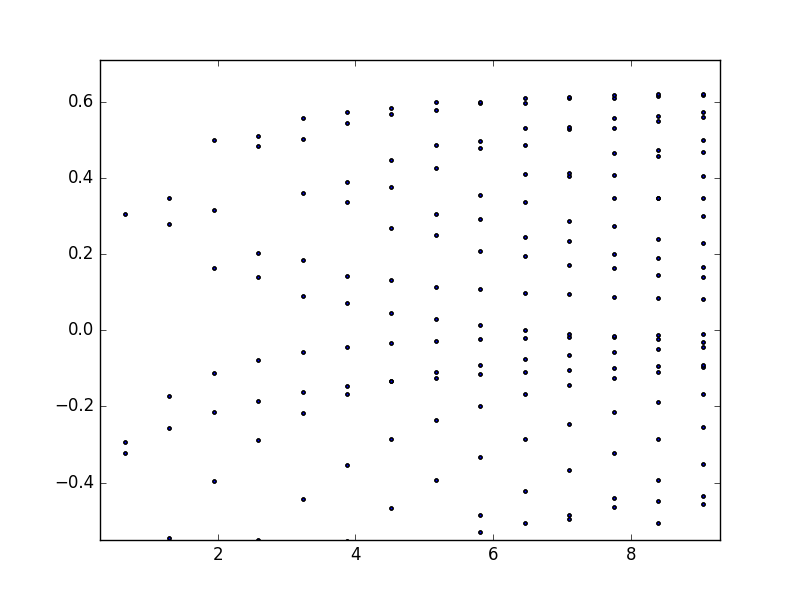
\includegraphics[width=0.8\linewidth]{dim_quant_levels.png}
    \caption{
            На графике изображены уровни размерного квантования, полученные 
            численной диагонализацией, для $k_x, k_y = 0$
            в зависимости от толщины слоя HgTe, nm. Видно, что два уровня размерного
            пересекаютcя при $d \approx 7.5$.
            }
\end{figure}

    \section{Топологический инвариант}
Кратко изложим, что представляет из себя TKNN--инвариант для произвольного 
зонного гамильтониана. Пусть гамильтониан системы в импульсном представлении даётся некоторой
матрицей $H(k)$, где $k$ --- волновой вектор зоны Бриллюэна.  
Для каждого $k$ гамильтониан всегда можно диагонализовать
и получить набор собственных векторов $u_i(k)$. Будем считать, что ни при каком $k$ нет 
вырождения спектра (это соответствует случаю изолятора). 
Выбор собственного базиса неоднозначен: каждый вектор
можно домножить на произвольную фазу. Очевидно, что в каждой окрестности $k$ можно выбрать
фазу каждого вектора так, чтобы она непрерывно зависела от $k$. Однако, вообще говоря, 
эту фазу может оказаться невозможно однозначно задать во всей зоне Бриллюэна.

Рассмотрим одну из ветвей спектра гамильтониана: $u_i(\vec{k})$ 
(в дальнейшем опустим индекс $i$). Предположим для простоты, что зону Бриллюэна
можно разбить на две части $A$ и $B$, 
в каждой из которых фазу $u(k)$  можно определить однозначно. 
Назовём функции Блоха в этих двух частях $u_a(k)$ и $u_b(k)$. На границе $A$ и $B$ (назовём
её $\gamma$) должно выполняться равенство
\begin{equation}
   u_b(k) = e^{-i\phi(k)}u_a(k).
\end{equation}
Определим число Черна, иначе называемое $\mathrm{TKNN}$--инвариант 
(см. \cite{Kohmoto1985, Thouless1982}), как
\begin{equation}
    \label{chern_number_definition}
    N = \frac{1}{2\pi}\int_\gamma d\phi
\end{equation}
С помощью простого вычисления %(используется формула Стокса) 
$N$ можно записать как интеграл по всей зоне Бриллюэна:
\begin{equation}
    N = \frac{1}{2\pi i}\int_\gamma \langle u_a |\vec{\nabla}_k u_a \rangle  - 
                             \langle u_b |\vec{\nabla}_k u_b \rangle d\vec{k} = 
        \frac{1}{2\pi i} 
            \int d^2 k\, \left[\partial_i \langle u | \partial_j u \rangle -
            \partial_j \langle u | \partial_i u \rangle \right]
\end{equation}
В последнем интеграле подыынтегральное выражение калибровочно--инвариантно, что
позволяет опустить индексы $a,b$. 

%Пусть $u(\vec{k})$ однозначно задана в зоне Бриллюэна, \emph{однако вместо периодических 
%граничных условий выполнены более слабые условия:} 
%\begin{equation}
%    \begin{gathered}
%        u(k_x, 2\pi) = e^{i\phi_x(k_x)} u(k_x, 0),\\
%        u(2\pi, k_y) = e^{i\phi_y(k_y)} u(0, k_y)
%    \end{gathered}
%\end{equation}
%Разумно считать, что это всегда возможно, так как квадрат топологически тривиален.
%В этом случае можно определить инвариант как оборот фазы $u(k)$ при движении по границе
%зоны Бриллюэна.

    \subsection{Модель сильной связи для топологического изолятора}
Можно написать эквивалентный гамильтониан сильной связи. Блок
для одной компоненты спина будет иметь следующий вид (для простоты предполагается симметрия
зон):
\begin{equation}
    \label{BHZ}
    H = \left(\begin{matrix}
            \xi + \frac{1}{m}(2 - \cos{p_x} - \cos{p_y}) & 2t(\sin{p_x} - i\sin{p_y})   \\
            2t(\sin{p_x} + i\sin{p_y}) & - \xi - \frac{1}{m}(2 - \cos{p_x} - \cos{p_y}) \\
        \end{matrix}\right)
\end{equation}
Спектр этого гамильтониана несложно вычислить:
\begin{equation}
    E_p^2 = (\xi + \frac{1}{m}(2 - \cos{p_x} - \cos{p_y}))^2 + 4t^2(\sin^2{p_x} + \sin^2{p_y})
\end{equation}
Как видно, гамильтониан описывает две симметричные зоны, щель между которыми равна $2|\xi|$. 
При малых $k$ $E_p^2 = \xi^2 + (4t^2 + \xi/m)k^2$, то есть спектр дираковский.

В координатном (решёточном) представлении гамильтониан выглядит так:
\begin{multline}
    \label{BHZ_tight_binding}
    H_{\mathrm{lattice}} = \sum_{mn} \left\{
        a_{mn}^\dagger\left( \left(\xi + \frac{2}{m}\right) a_{mn}
                 -\frac{1}{2m}(a_{m+1,n} + a_{m-1,n} + a_{m,n+1} + a_{m,n-1})\right)\right. \\
        -it a_{mn}^\dagger(b_{m+1,n} -b_{m-1,n} - i(b_{m,n+1} - b_{m,n-1}))\\
        -it b_{mn}^\dagger(a_{m+1,n} -a_{m-1,n} + i(a_{m,n+1} - a_{m,n-1}))\\
        -\left. b_{mn}^\dagger\left( \left(\xi + \frac{2}{m}\right) b_{mn}
                 -\frac{1}{2m}(b_{m+1,n} + b_{m-1,n} + b_{m,n+1} + b_{m,n-1})\right) \right\}
\end{multline}
Здесь $a_{mn}$, $b_{mn}$ --- операторы уничтожения состояний двух зон 
соответственно на узле $(m,n)$. Непосредственно обобщая этот решёточный гамильтониан, можно
рассматривать решётку конечного размера, добавлять примеси и так далее. 

    \subsection{Почему BHZ--модель описывает топологический изолятор}
Покажем, что модель \eqref{BHZ} действительно описывает топологический изолятор, то есть для
неё отличен от нуля TKNN--инвариант. 

Для определённости рассмотрим зону с $E>0$. Для волновой функции в этом случае существуют две
калибровки, $u(p)$ и $v(p)$:
\begin{multline}
    u(p) = \frac{1}{\sqrt{(E_p + \xi + \frac{2}{m}(2 - \cos{p_x} - \cos{p_y}))^2 + 
                        4t^2(\sin^2{p_x} + \sin^2{p_y})}} \times \\
                \begin{pmatrix}
                    \xi + \frac{2}{m}(2 - \cos{p_x} - \cos{p_y}) \\
                    2t(\sin{p_x} + i\sin{p_y})
                \end{pmatrix}
\end{multline}
\begin{multline}
   v(p) = \frac{1}{\sqrt{(E_p - \xi - \frac{2}{m}(2 - \cos{p_x} - \cos{p_y}))^2 + 
                        4t^2(\sin^2{p_x} + \sin^2{p_y})}} \times \\
                \begin{pmatrix}
                    -2t(\sin{p_x} + i\sin{p_y}) \\
                    \xi + \frac{2}{m}(2 - \cos{p_x} - \cos{p_y})
                \end{pmatrix}
\end{multline}
Легко видеть, что если $xi > 0$, то $u(p)$ определена для всеё зоны Бриллюэна, и,
следовательно, TKNN--инвариант обращается в ноль. Напротив, если $\xi < 0$, то
$u(p)$ не определена при $p = (0, 0)$, а $v(p)$ --- при $p = (\pi, \pi)$. При близких 
к нулю $p$ $u(p)$ приближённо равна
\begin{equation}
    u(p) \approx \begin{pmatrix}
                    0 \\
                    \frac{p_x + ip_y}{\sqrt{p_x^2 + p_y^2}}
                 \end{pmatrix}
\end{equation}
а $v(p)$ ---    
\begin{equation}
    u(p) \approx \begin{pmatrix}
                    0 \\
                    1
                 \end{pmatrix}
\end{equation}
Таким образом, $u(p) = v(p) e^{i\phi}$. В соответствии с определением 
\eqref{chern_number_definition}, следовательно, топологический инвариант равен $1$ (набег фазы
равен $2\pi$).

    \section{Краевые состояния}
Рассмотрим одномерную цепочку \eqref{ham1d} с возмущением \eqref{pert} и устремим $\Delta E$
к бесконечности. Физически это означает добавление бесконечно высокой потенциальной стенки,
в результате чего мы получаем две полуцепочки, не связанные между собой. Далее можно 
обычным способом искать локализованные состояния. (Они называются таммовскими, так 
как впервые были рассмотрены Таммом, см. \cite{Tamm1933}, \cite{Shockley1939})

Разумеется, сказанное относится не только к цепочке \eqref{ham1d}, но и к любой другой модели
сильной связи. Всегда можно ввести такое возмущение, которое разделит систему на две
несвязанные части. Например, в случае плоскости возмущение должно быть примерно таким:
\begin{equation}
	\hat{V} = \Delta E \sum_m a^\dagger_{m,0} a_{m,0}, \quad \Delta E \to \infty
\end{equation}
Это означает, что мы добавляем целую линию примесных атомов с очень большой энергией.

В частном случае гамильтониана \eqref{ham1d} функция Грина получается такой:
\begin{multline}
	G^R(\omega, m,n) = G^R_0(\omega, m,n) - 
		\frac{G^R_0(\omega, m,0)G^R_0(\omega, 0, n)}{G^R_0(\omega,0,0)} = \\
		= \frac{e^{-|m-n|\kappa} - e^{-|m|\kappa- |n|\kappa}}{2t\sinh \kappa}
\end{multline}
Здесь нет локализованных состояний: у функции Грина нет изолированных полюсов. Локализованные
состояния возникают в более сложных случаях, некоторые из которых будут рассмотрены ниже.

\section{Два примера одномерной цепочки}
Так как в самой простой цепочке локализованных состояний не оказалось, усложним цепочку.
А именно, рассмотрим цепочку чередующихся атомов с разными свойствами. 

Во--первых, можно рассмотреть цепочку, где все матричные элемементы перехода между 
соседними атомами одинаковы, а энергии атомов различаются. Гамильтониан такой цепочки ---
\begin{equation}
	H = \sum_n \xi(a_n^\dagger a_n - b_n^\dagger b_n) + ta_n^\dagger(b_n + b_{n-1}) +
			ta_n(b_n^\dagger + b_{n-1}^\dagger)
\end{equation}
Во--вторых, возможен случай, когда энергии атомов одинаковы, но, напротив, различаются 
матричные элементы. Гамильтониан в этом случае ---
\begin{equation}
	H = \sum_n t_1(a_n^\dagger b_n + a_n b_n^\dagger) + 
		t_2 (a_{n+1}^\dagger b_n + a_{n+1} b_n^\dagger)
\end{equation}
Оказывается, что краевое состояние есть только у второй цепочки, причём его наличие 
зависит от типа последней связи в решётке.

Рассмотрим подробнее вторую цепочку. Без ограничения общности будем считать, что
$t_1 > t_2 > 0$ .

После преобразования Фурье гамильтониан примет вид
\begin{equation}
	H = \sum_p 
			(t_1 e^{-\frac{ipa}{2}} + t_2 e^{\frac{ipa}{2}}) a_p^\dagger b_p + 
			(t_1 e^{\frac{ipa}{2}} + t_2 e^{-\frac{ipa}{2}}) a_p b_p^\dagger
\end{equation}
Отсюда получаем энергетический спектр, содержащий две зоны.
\begin{equation}
	E_p^{1,2} = \pm \epsilon_p = \pm|t_1 e^{\frac{ipa}{2}} + t_2 e^{-\frac{ipa}{2}}| = 
		\pm\sqrt{t_1^2 + t_2^2 + 2t_1t_2 \cos{pa}}
\end{equation}
Введём обозначение 
Гамильтониан диагонализуется преобразованием
\begin{equation}
	\left(
	\begin{matrix}
		a_p \\
		b_p
	\end{matrix}
	\right)
	=
	\frac12
	\left(
	\begin{matrix}
		1 & -e^{i\phi}	\\
		e^{-i\phi} & 1
	\end{matrix}
	\right)
	\left(
	\begin{matrix}
		x_p \\
		y_p
	\end{matrix}
	\right),
\end{equation}
\begin{equation}
	e^{i\phi} = \frac{t_1 e^{-\frac{ipa}{2}} + t_2 e^{\frac{ipa}{2}}}
				{\sqrt{t_1^2 + t_2^2 + 2t_1t_2 \cos{pa}}}
\end{equation}
Отсюда получаются выражения для функций Грина в импульсном представлении:
\begin{equation}
	\label{gaa}
	G^R_0 (\omega, p, A, A) =  G^R_0 (\omega, p, B, B) = \frac{1}{2}\left(
		\frac{1}{\omega - \epsilon_p + i\delta} + 
					\frac{1}{\omega + \epsilon_p + i\delta}\right)
\end{equation}
\begin{equation}
	G^R_0 (\omega, p, A, B) = \frac12 \left(\frac{e^{i\phi}}{\omega - \epsilon_p + i\delta} -
						\frac{e^{i\phi}}{\omega + \epsilon_p + i\delta} \right)
\end{equation}
\begin{equation}
	G^R_0 (\omega, p, B, A) = \frac12 \left(\frac{e^{-i\phi}}{\omega - \epsilon_p + i\delta} -
						\frac{e^{-i\phi}}{\omega + \epsilon_p + i\delta} \right)
\end{equation}
Здесь аргументы $A$, $B$ соответствуют операторам $a_p$ и $b_p$. 

Чтобы рассмотреть половину цепочки, введём возмущение 
$V = \Delta E a_0^\dagger a_0$, где $\Delta E$ очень велико.
Это приведёт к уже знакомому нам уравнению Дайсона. Его решение --- 
\begin{multline}
	G^R(\omega, m, s, n, s') = 
		G^R_0(\omega, m,s,n,s') - 
		\frac{G^R_0(\omega, m, s, 0, A)G^R_0(\omega, 0, A, n, s')}{G^R_0(\omega, 0, A, 0, A)},\\
		s,s' = A,B
\end{multline}
Уровни энергии даются, как видно, нулями функции $G^R_0(\omega, 0,A,0,A)$, а волновая функция
связанного состояния пропорциональна $G^R_0(\omega, m,s,0,A)$.

В нашем случае, как нетрудно убедиться, этот уровень энергии --- $E = 0$. Действительно, подставим 
$\omega = 0$ в (\ref{gaa}). Получается
\begin{equation}
	G^R_0 (\omega, p, A, A) = 
		-\frac{1}{2\epsilon_p} + 
					\frac{1}{2\epsilon_p} = 0
\end{equation}
Отсюда следует, что функции Грина в узельном представлении, 
составленные из операторов $a$, обращаются в нуль для всех $m,n$, и, таким образом, волновая 
функция связанного состояния равна нулю во всех узлах $a$. 

Волновая функция оказывается равной 
\begin{equation}
	\begin{split}
	\psi(n,A) &  = 0, \\
	\psi(n, B) & = 
	\left\{
	\begin{matrix}
		{\displaystyle
 		\sqrt{1 - \left(\frac{t_2}{t_1}\right)^2}(-1)^n \left(\frac{t_2}{t_1}\right)^n}
									&	\quad \mbox{при} \quad n \ge 0 \\
		0 & \quad \mbox{при} \quad n < 0
	\end{matrix}
	\right.,\\
	\end{split}
\end{equation}

Краевое состояние есть только у правой половины цепочки, у которой последнее перекрытие --- 
$t_2$, то есть маленькое.

Теперь рассмотрим цепочку с одинаковыми элементами перекрытия. Все вычисления для неё
проводятся точно так же, поэтому просто приведём их результаты:
\begin{equation}
	E_p^{1,2} = \pm \epsilon_p = \pm \sqrt{\xi^2 + 4t^2 \cos^2{\frac{pa}{2}}}
\end{equation}
\begin{equation}
	\begin{split}
	G_0^R(\omega, p, A, A) = \frac{\omega + \xi}{\omega^2 - \epsilon_p^2 + i\delta}\\
	G_0^R(\omega, p, A, B) = \frac{2t\cos{pa}}{\omega^2 - \epsilon_p^2 + i\delta}\\
	G_0^R(\omega, p, B, B) = \frac{\omega - \xi}{\omega^2 - \epsilon_p^2 + i\delta}\\
	\end{split}
\end{equation}
Уровни энергии для системы с возмущением 
определяются уравнением $G_0^R(\omega,0,A,0,A) = 0$, или 
{\sloppy

}

\begin{equation}
	0=\int_{-\pi}^{\pi} \frac{dk}{2\pi} 
		\frac{\omega + \xi}{\omega^2 - \xi^2 - 2t^2 - 2t^2\cos{pa} + i\delta} 
\end{equation}
Интеграл обращается в ноль при $\omega = -\xi$, на границе непрерывного спектра. Внутри
запрещённой зоны, то есть в области $|\omega| < \xi$, интеграл строго отрицателен. Отсюда
можно заключить, что в этом случае граничного состояния не существует: никаких новых
полюсов у функции Грина не возникло.

    \section{Точечная примесь}
Гамильтониан простейшего топологического изолятора может быть записан в виде
\begin{equation}
    \label{BHZ}
    H = \left(\begin{matrix}
            \xi + \frac{1}{m}(2 - \cos{p_x} - \cos{p_y}) & 2t(\sin{p_x} - i\sin{p_y})   \\
            2t(\sin{p_x} + i\sin{p_y}) & - \xi - \frac{1}{m}(2 - \cos{p_x} - \cos{p_y}) \\
        \end{matrix}\right)
\end{equation}
Уровни энергии ---
\begin{equation}
    E_p^2 = (\xi + \frac{1}{m}(2 - \cos{p_x} - \cos{p_y}))^2 + 4t^2(\sin^2{p_x} + \sin^2{p_y})
\end{equation}
Если перейти из импульсного представления в координатное, то он превратится в гамильтониан
сильной связи. Гамильтониан примеси тогда можно записать в виде
\begin{equation}
    V = \Delta E (a_{00}^\dagger a_{00} + b_{00}^\dagger b_{00})
\end{equation}
\subsection{Энергия связанных состояний}
Связанные состояния даются уравнением
\begin{equation}    
    \det{\left[\mathbbm{1} - \Delta E \int \frac{d^2 p}{(2\pi)^2} 
            \frac{\omega + \hat{H}}{\omega^2 - E_p^2}\right]} = 1
\end{equation}
В последнем интеграле (от матрицы) недиагональные члены из--за симметрии обращаются в ноль.
Таким образом, связанные состояния сводятся к уравнениям
\begin{equation}
    \label{integrals}
    \left[
    \begin{split}
        &\int \frac{d^2 p}{(2\pi)^2} 
            \frac{\omega + \xi + \frac{1}{m}(2 - \cos{p_x} - \cos{p_y})}
                 {\omega^2 - E_p^2} = \frac{1}{\Delta E},\\
        &\int \frac{d^2 p}{(2\pi)^2} 
            \frac{-\omega + \xi + \frac{1}{m}(2 - \cos{p_x} - \cos{p_y})}
                 {\omega^2 - E_p^2} = -\frac{1}{\Delta E},
    \end{split}
    \right.
\end{equation}
Эти интегралы можно взять приближённо в круге небольшого радиуса $p_{\mathrm{max}}$,
если учесть, что при малых $p$ спектр близок к 
коническому. После интегрирования получается
\begin{equation}
    G(\omega,0,0)_{11} = -\frac{1}{8\pi}\frac{1}{m(4t^2 + \frac{\xi}{m})}
        \left[ p_{\mathrm{max}}^2 + 
            \left(2m(\omega+\xi) - \frac{\xi^2 - \omega^2}{4t^2 + \frac{\xi}{m}}\right) 
                \log{\left(1 + \frac{\left(4t^2 + \frac{\xi}{m}\right)p_{\mathrm{max}}^2}
                                    {\xi^2 - \omega^2}\right)}\right]
\end{equation}
Конечно, интегралы из \eqref{integrals} можно взять численно. Для 
$\xi, m, t = -0.03, 0.1, 0.5$ компоненты функции Грина изображены на графике.

\begin{figure}[h]
    \centering
    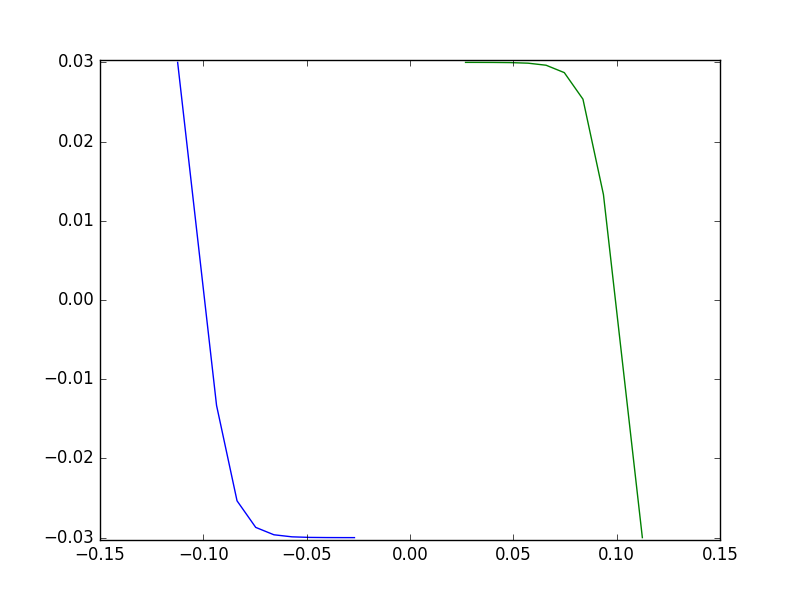
\includegraphics[width=0.8\linewidth]{impurity_levels.png}
    \caption{
            На графике показаны уровни энергии связанных состояний на точечной примеси. 
            По оси абсцисс отложена обратная глубина ямы, $\Delta E^{-1}$. <<Хвосты>>
            обоих графиков должны быть продолжены до бесконечности, у синего графика ---
            вправо снизу, у зелёного --- влево сверху. Видно,
            что при бесконечной глубине ямы имеются два слабо связанных состояния.
            }
\end{figure}

Вычисление выше показывает, что происходит на краях этого графика. А именно, ``хвосты'' 
функций Грина растут логарифмически до бесконечности.
Таким образом, для малых $\Delta E < 0$ появляется одно связанное состояние около 
зоны проводимости. При дальнейшем росте возмущения появляется состояние около валентной зоны.

\subsection{Волновые функции}
Волновые функции даются компонентами свободной
функции Грина:
\begin{equation}
    \Psi_{\alpha, i}(x) = G_0(x)_{\alpha i}
\end{equation}
Здесь $\alpha$ --- ``спинорный'' индекс, а $i$ --- индекс, соответствующий номеру волновой 
функции.

Функция Грина --- 
\begin{equation}
    G_0(x) = \int \frac{d^2 p}{(2\pi)^2} 
            \frac{\omega + \hat{H}}{\omega^2 - E_p^2} e^{ipx}
\end{equation}
Их можно вычислить с помощью формального трюка. Определим новую функцию
$F(x,y)$:
\begin{equation}
    F(x,y) = \equiv \int \frac{d^2 p}{(2\pi)^2} 
            \frac{e^{ip_x x + ip_y y}}{\omega^2 - E_p^2} 
\end{equation}
Несложно понять, что компоненты функций Грина выражаются (точными соотношениями)
 через $F(x,y)$. А именно,
\begin{equation}
    \label{differences}
    \begin{split}
        G_{11} & = (\omega + \xi) F(x,y) - 
            \frac{1}{m}(F(x+1,y) + F(x-1,y) + F(x,y+1) + F(x, y-1) - 4F(x,y))\\
        G_{21} & = -it(F(x+1,y) - F(x-1,y)) + t(F(x,y+1) - F(x,y-1))
    \end{split}
\end{equation}
С другой стороны, $F(x,y)$ может быть вычислена приближённо. Если разложить 
выражение в знаменателе около $p = 0$ и распространить интегрирование до $\infty$, то получится
сходящийся и берущийся интеграл.
\begin{equation}
    F(x,y) \approx -\int \frac{p\,dp\,d\cos{\theta}}{(2\pi)^2} 
        \frac{e^{ipr\cos{\theta}}}{\xi^2 - \omega^2 - (4t^2 + \frac{\xi}{m})p^2} = 
        -\frac{1}{2\pi} \frac{1}{4t^2 + \frac{\xi}{m}}
        K_0 \left(\sqrt{\frac{\xi^2 - \omega^2}{4t^2 + \frac{\xi}{m}}}R \right)
\end{equation}
Разности \eqref{differences} можно аппроксимировать производными. Пользуясь тем, что
$K_0(x)$ --- решение модифицированного уравнения Бесселя, получим 
\begin{equation}
    \begin{split}
        G_{11} & = -\frac{1}{2\pi} \frac{1}{4t^2 + \frac{\xi}{m}}
        \left( \omega + \xi - \frac{1}{m} \frac{\xi^2 - \omega^2}{4t^2 + \frac{\xi}{m}} \right)
        K_0 \left(\sqrt{\frac{\xi^2 - \omega^2}{4t^2 + \frac{\xi}{m}}}R \right)\\
        G_{21} & = \frac{it}{\pi} \sqrt{\frac{\xi^2 - \omega^2}
                                     {(4t^2 + \frac{\xi}{m})^{3}}}
        K_0' \left(\sqrt{\frac{\xi^2 - \omega^2}{4t^2 + \frac{\xi}{m}}}R \right)e^{i\theta}
    \end{split}
\end{equation}
%Найдём момент импульса найденных состояний. Оператор полного момента имеет вид
%\begin{equation}
%    J_z = x p_y - y p_x + \frac{1}{2}\sigma_z
%\end{equation}
%Несложно понять, что у двух найденных состояний полный момент равен $\pm \frac{1}{2}$.
%
%Интересно также найти магнитный момент. Оператор магнитного момента ---
%\begin{equation}
%    m_z = \frac{e}{2c}(x v_y - y v_x) + \frac{e}{2m_0c} \sigma_z
%\end{equation}
%Операторы скорости в низшем порядке по импульсам ---
%\begin{equation}
%    \begin{split}
%        v_x & = \begin{pmatrix} 
%                -\frac{i}{m} \partial_ x & 2t \\
%                2t & \frac{i}{m}\partial_x
%              \end{pmatrix} \\
%        v_y & = \begin{pmatrix} 
%                -\frac{i}{m} \partial_y & -2it \\
%                2it & \frac{i}{m}\partial_y
%              \end{pmatrix} \\
%    \end{split}
%\end{equation}
%Таким образом,
%\begin{equation}
%    m_z = \frac{e}{2mc}
%            \begin{pmatrix}
%               l_z & -2imt\cdot re^{-i\theta} \\
%               2imt\cdot r e^{i\theta} & -l_z
%            \end{pmatrix} + 
%          \frac{e}{2m_0c} \sigma_z
%\end{equation}

%    \section{Численная диагонализация решёточного\\ гамильтониана}
Как уже говорилось, краевые состояния не рассеиваются на потенциальном беспорядке, 
если нет объёмных или примесных состояний с той же энергией. 
Это можно увидеть непосредственно, 
диагонализуя решёточный гамильтониан. Из результатов численной диагонализации видно, что
краевые состояния огибают глубокое препятствие (см. рис.~\ref{fig:obstacle}).
\begin{figure}[h]
    \centering
    \begin{minipage}[t]{0.4\linewidth}
        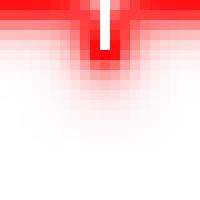
\includegraphics[width=0.9\linewidth]{obstacle_1.png}
    \end{minipage}
    \hfill
    \begin{minipage}[t]{0.4\linewidth}
        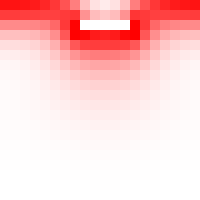
\includegraphics[width=0.9\linewidth]{obstacle_2.png}
    \end{minipage}
    \caption{
        Квадрат амплитуды волновой функции краевого состояния, огибающего препятствия. 
        Размер решётки --- $20\times20$, по горизонтальной оси наложены периодические
        граничные условия.
    }
    \label{fig:obstacle}
\end{figure}

Также краевые состояния <<выживают>> под действием даже довольно сильного потенциального
беспорядка
\begin{equation}
    \hat{V} = \sum_{m,n} V_{mn} (a_{mn}^\dagger a_{mn} + b_{mn}^\dagger b_{mn}),
\end{equation}
где $V_{mn}$ равномерно распределены по отрезку $[-\frac{W}{2}, \frac{W}{2}]$, см.
рис.~\ref{fig:disordered_stripe}.

\begin{figure}[h]
    \centering
    \begin{minipage}[h]{0.4\linewidth}
        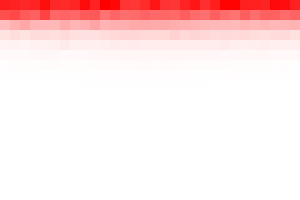
\includegraphics[width=1.\linewidth]{dis_edge_state_1.png}
        \caption{
            Волновая функция краевого состояния с беспорядком.
            Параметры модели: $\xi, m, t = -0.2, 1, 0.4$, сила беспорядка --- $0.5$.
            }
    \end{minipage}
    \hfill
    \begin{minipage}[h]{0.4\linewidth}
        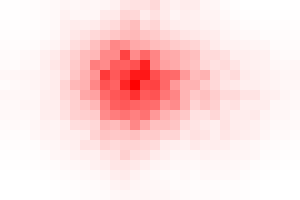
\includegraphics[width=1.\linewidth]{dis_bulk_state.png}
        \caption{
            Волновая функция объемного состояния с беспорядком для тех же параметров.
            }
    \end{minipage}
    \label{fig:disordered_stripe}
\end{figure}

Магнитный беспорядок, как нарушающий $T$--симметрию, приводит к рассеянию состояний
с двумя компонентами спина друг в друга. Это приводит к локализации краевых состояний,
что продемонстрировано на рис.~\ref{fig:magnetic_disorder}.  Магнитный беспорядок 
в симуляции имел вид
\begin{equation}
    \hat{V}_{\mathrm{mgn}} = \sum_{mn} J \hat{\sigma}_{mn} S_{mn},
\end{equation}
$\hat{\sigma}$ --- оператор спина на узле, $S_{mn}$ --- случайный вектор на единичной сфере.
\begin{figure}[h]
    \centering
    \begin{minipage}[h]{0.9\linewidth}
        \centering
        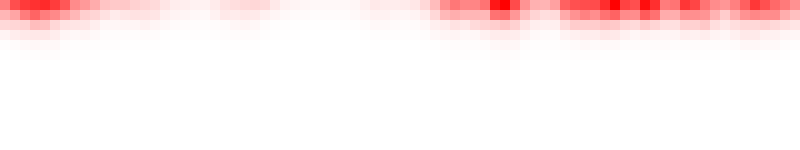
\includegraphics[width=0.7\linewidth]{mgn_edge_st_1.png}
    \end{minipage}
    \vfill
    \begin{minipage}[h]{0.9\linewidth}
        \centering
        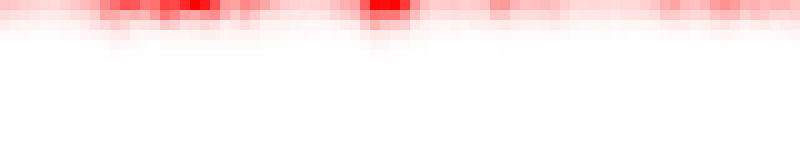
\includegraphics[width=0.7\linewidth]{mgn_edge_st_2.png}
    \end{minipage}
    \vfill
    \begin{minipage}[h]{0.9\linewidth}
        \centering
        
\includegraphics[width=0.7\linewidth]{mgn_edge_st_3.png}
    \end{minipage}
    \caption{
        Волновые функции краевых состояний с магнитным беспорядком 
        для тех же параметров.
        }
    \label{fig:magnetic_disorder}
\end{figure}

Также мы диагонализовали гамильтониан для случая, когда энергии примесных состояний
лежат в середине щели (см. рис.~\ref{fig:impurity_numeric_levels}). Для этого нужно
специальным образом подобрать силу возмущения.

\begin{figure}[h]
    \centering
    \begin{minipage}[h]{0.9\linewidth}
        \centering
        
\includegraphics[width=0.7\linewidth]{fig2.png}
    \end{minipage}
    \vfill
    \begin{minipage}[h]{0.9\linewidth}
        \centering
        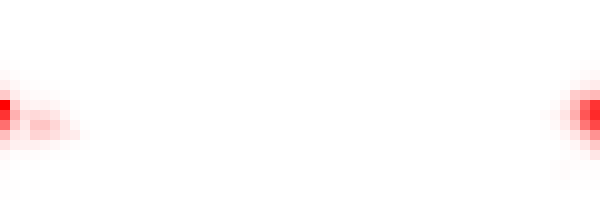
\includegraphics[width=0.7\linewidth]{fig3.png}
    \end{minipage}
    \vfill
    \begin{minipage}[h]{0.9\linewidth}
        \centering
        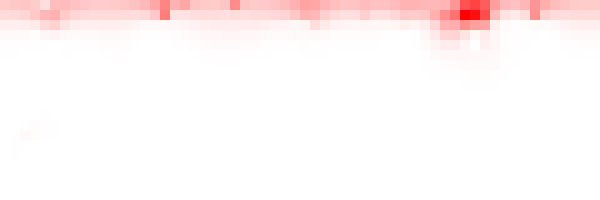
\includegraphics[width=0.7\linewidth]{fig5.png}
    \end{minipage}
    \caption{
        Волновые функции краевых состояний c примесями внутри щели      
    }

    \label{fig:magnetic_disorder}
\end{figure}

    \documentclass{article}
\usepackage{amsmath}
\usepackage{graphicx}
\usepackage[utf8]{inputenc}
\usepackage[T1, T2A]{fontenc}
\usepackage[english,russian]{babel}

\title{Теория рассеяния}
\author{Anikin Evgeny, 121}

\begin{document}
\maketitle
\section{$S$--матрица и амплитуда рассеяния}
\begin{multline}
    \Psi(x,t) = \int \frac{dk}{2\pi} \phi(k)\left(e^{ikz} + \frac{f(\theta)}{r}e^{ikr}\right)
                e^{-\frac{i\hbar k^2t}{2m} + ikR} = \\
               = \phi\left(\frac{m(r+R)}{\hbar t}\right) \frac{f(\theta)}{r}
                e^{\frac{im(r+R)^2}{2\hbar t}} \sqrt{\frac{m}{2\pi i\hbar t}}
\end{multline}
Здесь и далее считаем, что $\Re{\sqrt{z}} > 0$.

Далее сделаем преобразование Фурье:
\begin{equation}
   \Psi(\vec{k}) = \int d^3x\, e^{-i\vec{k}\vec{x}} \Psi(x,t) = 
    \int d^3x\, e^{-i\vec{k}\vec{x}}\phi\left(\frac{m(r+R)}{\hbar t}\right) \frac{f(\theta)}{r}
                e^{\frac{im(r+R)^2}{2\hbar t}} \sqrt{\frac{m}{2\pi i\hbar t}}
\end{equation}
Точка стационарной фазы ---
\begin{equation}
    \vec{k} = \frac{m(r+R)}{\hbar t} \vec{n},
\end{equation}
матрица вторых производных ---
\begin{equation}
    \partial_i \partial_j \frac{im(r+R)^2}{2\hbar t} = \frac{im}{\hbar t} 
                \left(\left(1 + \frac{R}{r}\right)\delta_{ij} - \frac{R}{r} n_i n_j\right)
\end{equation}
С помощью метода стационарной фазы получаем
\begin{equation}
    \Psi(\vec{k}) =  \frac{2\pi i}{k} \phi(k)  f(\theta) e^{-\frac{i\hbar k^2t}{2m} + ikR}
\end{equation}
Теперь уже можно положить $\phi(k) = \delta(k - k_0)$. Тогда, пользуясь формулой 
\begin{equation}
    \delta(k - k_0) = \frac{\hbar^2 k_0}{m} \delta(\epsilon - \epsilon_0),
\end{equation}
получим окончательно
\begin{equation}
    \Psi(\vec{k}) = \frac{2\pi i \hbar^2}{m} f(\theta) \delta(\epsilon - \epsilon_0)
\end{equation}
\section{Квазиклассическое приближение}
\subsection{Функция Эйри}
Функция Эйри --- решение уравнения
\begin{equation}
	u'' = xu
\end{equation}
Оно решается методом Лапласа, его решение ---
\begin{equation}
	u = \oint_\Gamma e^{ixz - \frac{iz^3}{3}}\,dz
\end{equation}
Контур $\Gamma$ должен начинаться и заканчиваться на бесконечности, так, чтобы 
$e^{-\frac{iz^3}{3}} \to 0$. Выберем его так, чтобы он шёл из третьей координатной четверти
к нулю и уходил на бесконечность вдоль $Ox$. Тогда 
\begin{equation}
	\Psi = \frac{\sqrt{\pi}}{|x|^{\frac14}}\left\{ \begin{matrix}
			e^{\frac23 x^{\frac32}}, & \quad x \gg 0 \\
			e^{\frac{2i}{3} |x|^{\frac32} + \frac{i\pi}{4}}, & \quad x \ll 0
			\end{matrix} \right.
\end{equation}
Методом перевала можно вычислить и мнимую часть $\Psi$. 
\begin{equation}
	\operatorname{Im}\Psi = \frac{\sqrt{\pi}}{|x|^{\frac14}}\left\{ \begin{matrix}
			\frac12 e^{-\frac23 x^{\frac32}}, & \quad x \gg 0 \\
			\sin{\left(\frac{2}{3} |x|^{\frac32} + \frac{\pi}{4}\right)}, & \quad x \ll 0
			\end{matrix} \right.
\end{equation}
\section{Квазиклассическая волновая функция}

\section{Разложение плоской волны по сферическим}
Для начала необходимо разложить плоскую волну по сферическим.
\begin{equation}
	e^{i\vec{k}\vec{r}} = e^{ikr\cos{\theta}} = \sum_l A_l(kr) P_l(\cos{\theta})
\end{equation}
Перепишем это разложение несколько в другом виде:
\begin{equation}
	e^{ixy} = \sum_l A_l(x) P_l(y)
\end{equation}
Отсюда
\begin{equation}
	A_l(x) = \frac{2l+1}{2} \int_{-1}^{1} P_l(y) e^{ixy} \, dy
\end{equation}
Вспоминаем формулу для полиномов Лежандра:
\begin{equation}
	P_l(y) = \frac{1}{2^l l!} \frac{d^l}{dy^l} (y^2 - 1)^l
\end{equation}
Тогда после подстановки и $n$--кратного интегрирования по частям получим 
\begin{equation}
	A_l(x) = \frac{(2l+1)(ix)^l}{2} \int_{-1}^{1} (1-y^2)^l e^{ixy} \, dy
\end{equation}
Здесь нас интересует случай больших $x$. Основной вклад в интеграл дают окрестности 
$y = \pm 1$ (можно деформировать контур так, чтобы это стало совсем очевидно).
{ \it Интересно, как точно вычислить этот интеграл? Ответ тут мне известен аж в двух
смыслах: во--первых, интеграл сводится к вырожденной гипергеометрии, 
во-вторых, должны получиться
функции Бесселя полуцелого порядка. }

После вычисления асимптотики получается следующий результат:
\begin{equation}
    e^{ixy} = \sum \frac{2l+1}{2ix} \left[ e^{ix} + (-1)^{l+1} e^{-ix} \right] P_l(y)
\end{equation}

\section{Задача рассеяния}
Пусть $R_l(r)$ --- радиальные функции. Так как на больших расстояниях потенциала нет,
они имеют асимптотический вид
\begin{equation}
    R_l(r) \approx \frac{1}{r}\left(e^{ikr} + (-1)^{l+1}e^{-ikr-i\alpha_l}\right)
\end{equation}
(Множитель $(-1)^{l+1}$ выбран для удобства в последующем.)    

Любая функция с цилиндрической симметрией должна представляться в виде
\begin{equation}
    \label{expansion}
    \Psi(r,\theta) = \sum_l R_l(r) P_l(\cos{\theta})
\end{equation}
Пусть плоская волна падает на рассеивающий центр. Тогда волновая функция имеет вид
\begin{equation}
    \Psi(r,\theta) = e^{ikr\cos{\theta}} + \frac{f(\theta)e^{ikr}}{r}
\end{equation}
Используя разложение плоской волны и \eqref{expansion}, можно найти $f(\theta)$. Ответ
получается таким:
\begin{equation}
    f(\theta) = \sum_l \frac{2l+1}{2ik} (e^{i\alpha_l} - 1) P_l(\cos{\theta})
\end{equation}

\section{Рассеяние в квазиклассическом случае}

\section{Рассеяние на непроницаемой сфере}
Непроницаемая сфера, возможно, --- единственный случай, когда радиальные функции можно
вычислить точно. Они являются линейными комбинациями функций Бесселя полуцелого порядка.

\end{document}

    \newpage
\section{Заключение}
Краевые состояния оказываются устойчивыми не просто к слабому потенциальному беспорядку, 
но и к беспорядку, создающему ненулевую плотность состояний в щели. 

    \newpage
    \appendix
    \newpage
\section{Уровни размерного квантования\\ в квантовой яме HgTe}
\label{app:dim_quant}
Гамильтониан Кейна имеет вид
\begin{equation}
    \label{kane_ham}
    H = \begin{pmatrix}
                E_c + \frac{\hbar^2 k^2}{2m_s}E_{2\times 2} & T \\
                T^\dagger & E_v + H_{L}
        \end{pmatrix}
\end{equation}
\begin{equation*}
    H_L = -\frac{\hbar^2}{2m_0}\left[
            \left(\gamma_1 + \frac{5}{2}\gamma_2\right)k^2 -
            2\gamma_2(\vec{k} \cdot \vec{J})^2 - \right. 
            - \left.2(\gamma_3 - \gamma_2)(\{J_x J_y\} + \{J_x J_z\} + \{J_y J_z\})
            \vphantom{\frac{1}{2}}\right]
\end{equation*}
\begin{equation*}
    T = P\begin{pmatrix}
           -\frac{1}{\sqrt{2}}k_{+} & \sqrt{\frac{2}{3}}k_z  
                    & \frac{1}{\sqrt{6}} k_{-} & 0 \\
            0 & -\frac{1}{\sqrt{6}} k_{+} 
                    & \sqrt{\frac{2}{3}}k_z & \frac{1}{\sqrt{2}} k_{-} 
         \end{pmatrix}
\end{equation*}
Так как
коэффициенты в гамильтониане Кейна зависят явным образом от $z$, нужно сделать замену
$k_z \to i\partial_z$. При этом, чтобы гамильтониан остался эрмитовым,
$\frac{k_z^2}{2m} \to -\partial_z \frac{1}{2m} \partial_z$ (и аналогично --- для других
членов). Все величины, зависящие от $z$, равны значениям для HgTe при $-d/2 < z < d/2$,
для CdTe --- в противном случае.

Уровни размерного квантования можно относительно просто найти для $k_x, k_y = 0$. В этом 
случае гамильтониан значитально упрощается. Уровни тяжёлых дырок оказываются полностью
отщеплёнными для каждой проекции спина и описываются эффективным гамильтонианом
\begin{equation}
    H_{\mathrm{HH}} = E_v(z) + \frac{1}{2m}
                        \frac{\partial}{\partial z} 
                        (\gamma_1(z) - 2\gamma_2(z)) 
                        \frac{\partial}{\partial z} 
\end{equation}
Также отщепляются $s$--зона вместе с зоной лёгких дырок. Они описываются эффективным
гамильтонианом 
\begin{equation}
    H_{\mathrm{s,LH}} = \begin{pmatrix}
                            E_c - \frac{\hbar^2}{2m}
                                 \frac{\partial}{\partial z}(1 + 2F) 
                                 \frac{\partial}{\partial z} &
                                 \sqrt{\frac{2}{3}}P k_z \\
                                 \sqrt{\frac{2}{3}}P k_z &
                                 E_v +  \frac{\hbar^2}{2m}
                                 \frac{\partial}{\partial z}(\gamma_1 + 2\gamma_2)
                                 \frac{\partial}{\partial z} 
                        \end{pmatrix}
\end{equation}
Для обоих гамильтонианов можно получить алгебраические уравнения на уровни энергии. Эти
уравнения решаются численно.

    \section{Отсутствие рассеяния для крамерсовского дублета}
\label{app:kramers_doublet}
Нетрудно проверить, что для частицы со спином $\frac{1}{2}$
\begin{equation}
    \bra \chi | T\psi \ket = -\bra \psi | T\chi\ket
\end{equation}
Тогда $\bra \psi | \hat{A}  | T\psi \ket = 0$ для любого 
$|\psi \ket$, если
$\hat{A}$ удовлетворяет условию $-T\hat{A}^\dagger T = \hat{A}$.
Действительно,
\begin{equation}
    \bra \psi | \hat{A}  | T\psi \ket = \bra \hat{A}^\dagger \psi | T\psi \ket = 
       -\bra \psi | T \hat{A}^\dagger| \psi \ket = -\bra \psi | (-T\hat{A}^\dagger T) | T\psi \ket
\end{equation}
Оператор эволюции $T$--инвариантной системы удовлетворяет именно такому условию:
\begin{equation}
    -T\hat{U}T = U^{-1} = U^\dagger
\end{equation}
Поэтому рассеяние $|\psi\ket$ и $|T\psi\ket$ друг в друга запрещено.

    \section{Вычисления для точечной примеси}
\subsection{Энергия связанного состояния}
\label{app:impurity}
Уравнения \eqref{imp_equation} принимают вид
\begin{align}
        &G(\omega,0,0)_{11} = \int \frac{d^2 p}{(2\pi)^2} 
            \frac{\omega + \xi + \frac{1}{m}(2 - \cos{p_x} - \cos{p_y})}
                 {\omega^2 - E_p^2} =\frac{1}{\Delta E}, \label{local_state_eq:1}\\
        &G(\omega,0,0)_{22} = \int \frac{d^2 p}{(2\pi)^2} 
            \frac{-\omega + \xi + \frac{1}{m}(2 - \cos{p_x} - \cos{p_y})}
                 {\omega^2 - E_p^2} =-\frac{1}{\Delta E}, \label{local_state_eq:2}
\end{align}
Интегралы можно взять приближённо в круге радиуса $p_{\mathrm{max}}$,
если учесть, что при малых $p$ спектр близок к 
коническому. Можно считать, что $p_{\mathrm{max}} \sim 1$. После интегрирования получается
выражение \eqref{approx_green_func}. Используя его, мы получили \eqref{impurity_energy}.


Покажем, что для большого $\Delta E$ и $\xi > 0$ связанного состояния в щели нет. 
В этом случае $\delta \omega < 0$ и логарифм в формуле \eqref{approx_green_func} ---
большое положитальное число. При этом в правой части \eqref{local_state_eq:1} стоит
$\frac{1}{\Delta E} \to 0$. Это значит, что равенство не может быть выполнено.


\subsection{Волновая функция связанного состояния}
Волновые функции даются компонентами свободной функции Грина \eqref{green_function}.
Их можно вычислить с помощью формального трюка. Определим новую функцию
$F(x,y)$:
\begin{equation}
    F(x,y) = \equiv \int \frac{d^2 p}{(2\pi)^2} 
            \frac{e^{ip_x x + ip_y y}}{\omega^2 - E_p^2} 
\end{equation}
Несложно понять, что компоненты функций Грина выражаются (точными соотношениями)
 через $F(x,y)$. А именно,
\begin{equation}
    \label{differences}
    \begin{split}
        G_{11} & = (\omega + \xi) F(x,y) - 
            \frac{1}{m}(F(x+1,y) + F(x-1,y) + F(x,y+1) + F(x, y-1) - 4F(x,y))\\
        G_{21} & = -it(F(x+1,y) - F(x-1,y)) + t(F(x,y+1) - F(x,y-1))
    \end{split}
\end{equation}
С другой стороны, $F(x,y)$ может быть вычислена приближённо. Если разложить 
выражение в знаменателе около $p = 0$ и распространить интегрирование до $\infty$, то получится
сходящийся и берущийся интеграл.
\begin{equation}
    F(x,y) \approx -\int \frac{p\,dp\,d\cos{\theta}}{(2\pi)^2} 
        \frac{e^{ipr\cos{\theta}}}{\xi^2 - \omega^2 - (4t^2 + \frac{\xi}{m})p^2} = 
        -\frac{1}{2\pi} \frac{1}{4t^2 + \frac{\xi}{m}}
        K_0 \left(\sqrt{\frac{\xi^2 - \omega^2}{4t^2 + \frac{\xi}{m}}}R \right)
\end{equation}
Разности \eqref{differences} можно аппроксимировать производными. Пользуясь тем, что
$K_0(x)$ --- решение модифицированного уравнения Бесселя, получим 
\begin{equation}
    \begin{split}
        G_{11} & = -\frac{1}{2\pi} \frac{1}{4t^2 + \frac{\xi}{m}}
        \left( \omega + \xi - \frac{1}{m} \frac{\xi^2 - \omega^2}{4t^2 + \frac{\xi}{m}} \right)
        K_0 \left(\sqrt{\frac{\xi^2 - \omega^2}{4t^2 + \frac{\xi}{m}}}R \right)\\
        G_{21} & = \frac{it}{\pi} \sqrt{\frac{\xi^2 - \omega^2}
                                     {(4t^2 + \frac{\xi}{m})^{3}}}
        K_0' \left(\sqrt{\frac{\xi^2 - \omega^2}{4t^2 + \frac{\xi}{m}}}R \right)e^{i\theta}
    \end{split}
\end{equation}

    \section{Задача рассеяния}
\label{app:kwant}
Задача рассеяния ставится таким образом:
к системе, описываемой гамильтнианом $H_s$, присоединяются трансляционно--инвариантные 
контакты. Любой набор контактов можно описать, задав элементарную ячейку с гамильтонианом 
$H_L$ и матрицу перехода между ячейками $V_L$. Кроме того, нужно задать матрицу перехода
между системой и контактами. Полный гамильтониан системы с контактами
принимает вид
\begin{equation}
    H = \begin{pmatrix}
            H_S             & V_{LS}     & 0           & \ddots \\
            V_{LS}^\dagger  & H_L        & V_L         & 0  \\
            0               & V_L^\dagger& H_L         & V_L    \\
            \ddots          & 0          & V_L^\dagger & \ddots \\
        \end{pmatrix}
\end{equation}
Задачу рассеяния для такого гамильтониана можно свести к неоднородной системе линейных 
уравнений, которая может быть эффективно решена численно. Такой подход оказывается 
гораздо выгоднее, чем диагонализация гамильтониана $H_S$. 

Покажем, как свести задачу рассеяния к системе линейных уравнений. 
Волновая функция в задаче рассеяния имеет вид 
\begin{equation}
    \Psi = (\Psi_S, \Psi_V(0), \Psi_V(1), \dots)
\end{equation}
Так как контакты трансляционно инвариантны, $\Psi_V(k)$ можно искать в виде суперпозиции
плоских волн: $\Psi_V(k) = \Psi_V e^{ipk}$. Квазиимпульсы и волновые функции определяются 
уравнениями
\begin{equation}
    \label{modes}
    \begin{gathered}
        (V_L^\dagger e^{-ip} + H_L + V_L e^{ip} - E) \Psi_V = 0\\
        \det{(V_L^\dagger e^{-ip} + H_L + V_L e^{ip} - E)} = 0
    \end{gathered}
\end{equation}
Если размер матрицы $H_L$ --- $l$, то у уравнений \eqref{modes} будет $2l$ решений, из 
которых $l$ соответствуют падающим либо растущим волнам, а $l$ --- исходящим либо 
затухающим.

Пусть волновая функция рассеяния в контактах имеет вид
\begin{equation}
    \Psi_L(k) = \Psi_m e^{-ip_m k} + \sum_{n} r_{mn} \Psi_n e^{ip_n k}
\end{equation}
Здесь $m$ соответствует падающей моде, а $n$ --- затухающим либо исходящим волнам. Волновая 
функция $\Psi_S$ в регионе рассеяния, разумеется, тоже неизвестна. Подставляя волновую функцию
в уравнение Шрёдингера, получим уравнения на $\Psi_S$ и $r_{mn}$.
\begin{equation}
    \begin{gathered}
        H_S \Psi_S + \sum_n r_{mn} V_{LS} \Psi_n = -V_{LS} \Psi_m\\
        V_{LS}^\dagger\Psi_S  - \sum_n r_{mn}V_L \Psi_n e^{-ip_n} = V_L e^{ip_m} \Psi_m
    \end{gathered}
\end{equation}
Легко убедиться, что здесь уравнений столько же, сколько неизвестных, и систему можно решить.

Описанный метод решения задачи рассеяния используется в пакете Kwant \cite{Groth2014}.

    \newpage
    \bibliography{/home/ksenia/notes/science/top_ins/literature.bib}
\end{document}
